\documentclass[10pt,a4paper,final]{report}
\usepackage[latin1]{inputenc}
\usepackage{amsmath}
\usepackage{amsfonts}
\usepackage{amssymb}
\usepackage{graphicx}
\usepackage{listings}


\title{Miniproject 1 - DIS}
\author{Lars Andersen, Mathias Winde Pedersen \& S�ren Skibsted Als}
\begin{document}
	\maketitle
	\section*{B}
	By looking at the data, different business processes have been considered.
	A central one is that of sale.
	Another process to model is the payment process, which is the pre-insertion of money.
	
	We choose to focus on the sale business process.
	
	For the granularity, the data already contains a timestamp for each sale, as of such we maintain that granularity.
	
	
	That is timestamp without timezone, containing year, month, day, hour, minute and second.
	However, a weekday could be relevant as well, and when extracting the data, it could be interesting to include this information, same goes for season, holidays, and week number.
	
	The granularity for a member is year, as we cannot go deeper there, without coming up with some fictive data.
	
	The choices are reasonable for paying customers, which is reflected in the questions that can be asked.
	
	For sales, it could be interesting to see if the sales increase during breaks, and the granularity here is fine with down to minutes, for seconds it is still fine as it does not require much effort to record this as well.
	
	For member creation the year of creation is as close as we can get, thus this is also reasonable for the given data.
	
	\textbf{Questions that can be asked:}
	
	Does sales increase during break times (12:00 to 12:30)?
	
	How has the total sales per year evolved?
	
	Which product has been sold the most?
	
	Which member spends the most money?
	
	Which weekday, weeknumber, season, holiday have the largest revenue?
	
	
	\section*{C}
	For SCDs products could be useful, as the price changes slowly over time, same goes for members, as they can be active or inactive.
	
	For the time dimension, we skipped weekdays etc. as we would have to find a library of some sort to translate this.
	The dimensions have been specified in Figure \ref{fig:dimensions}. The schema can be seen in the code below and in Figure \ref{fig:schema}.
	
	\begin{figure}[h]
		\centering
		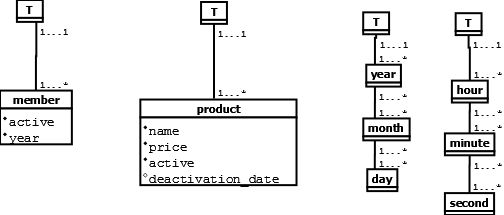
\includegraphics[scale=0.5]{dimensions}
		\caption{Dimensions, part C.}
		\label{fig:dimensions}
	\end{figure}
	
	\newpage
	\lstinputlisting[language=SQL]{codeschema.txt}
	
	\begin{figure}[h]
		\centering
		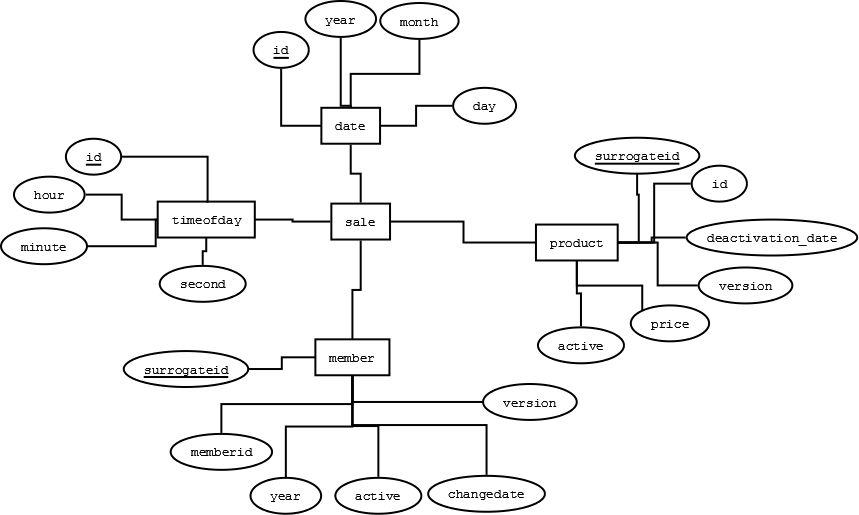
\includegraphics[scale=0.3]{starscheme}
		\caption{schema, part C.}
		\label{fig:schema}
	\end{figure}
	
\end{document}